

\begin{figure}[t]
     \centering
     \begin{subfigure}[b]{0.3\textwidth}
         \centering
         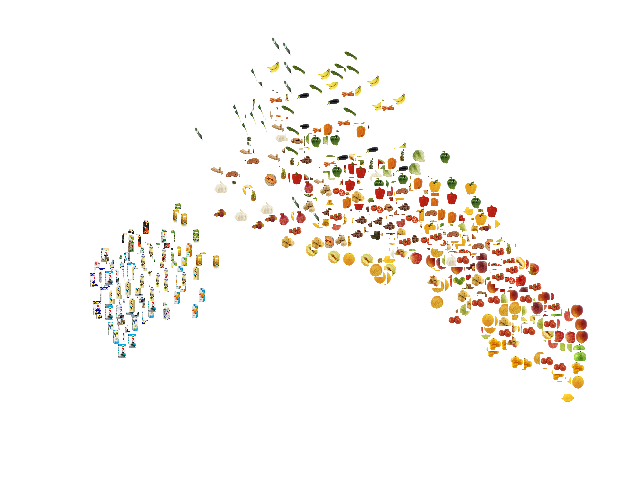
\includegraphics[width=\textwidth]{PaperB/figures_and_tables/latent_space_visualizations/pca_densenet.png}
         \caption{DenseNet169}
         \label{fig:pca_densenet}
     \end{subfigure}
     \begin{subfigure}[b]{0.3\textwidth}
         \centering
         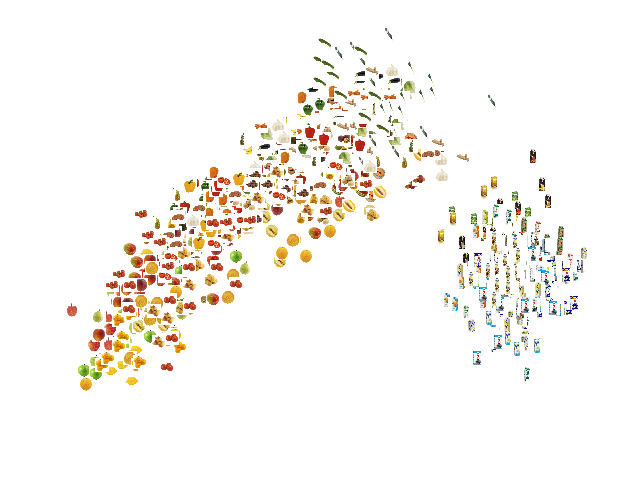
\includegraphics[width=\textwidth]{PaperB/figures_and_tables/latent_space_visualizations/pca_latents_vae_seed2.png}
         \caption{VAE$_{x}$}
         \label{fig:pca_vae_x}
     \end{subfigure} 
     \begin{subfigure}[b]{0.3\textwidth}
         \centering
         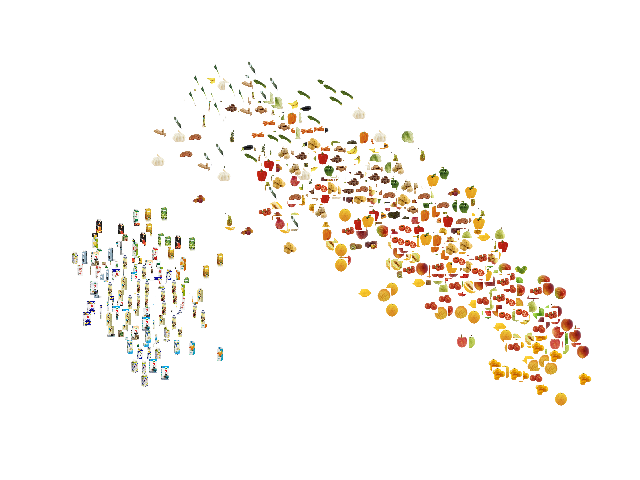
\includegraphics[width=\textwidth]{PaperB/figures_and_tables/latent_space_visualizations/pca_latents_vcca_xy_seed2.png}
         \caption{VCCA$_{x y}$}
         \label{fig:pca_vcca_xy}
     \end{subfigure} \\
     \begin{subfigure}[b]{0.3\textwidth}
         \centering
         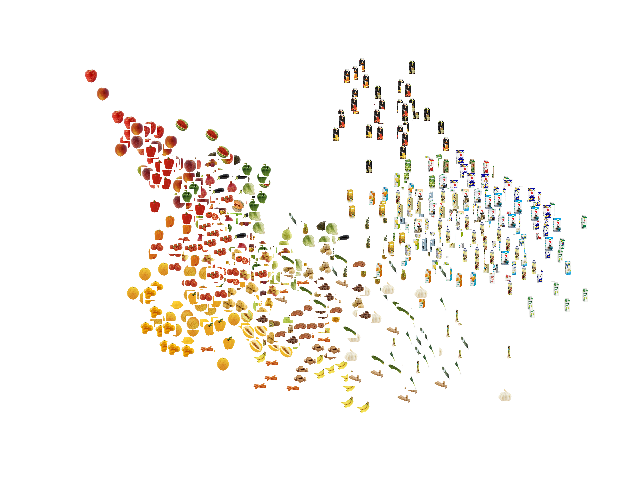
\includegraphics[width=\textwidth]{PaperB/figures_and_tables/latent_space_visualizations/pca_latents_vcca_xi_seed2.png}
         \caption{VCCA$_{x i}$}
         \label{fig:pca_vcca_xi}
     \end{subfigure} 
     \begin{subfigure}[b]{0.3\textwidth}
         \centering
         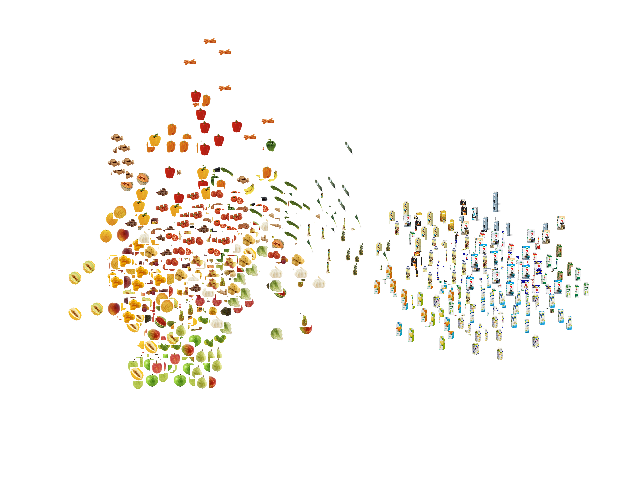
\includegraphics[width=\textwidth]{PaperB/figures_and_tables/latent_space_visualizations/pca_latents_vcca_xw_seed2.png}
         \caption{VCCA$_{x w}$}
         \label{fig:pca_vcca_xw}
     \end{subfigure} 
     \begin{subfigure}[b]{0.3\textwidth}
         \centering
         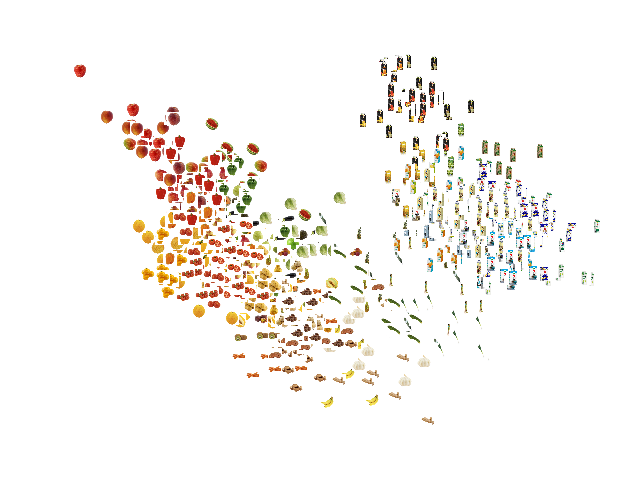
\includegraphics[width=\textwidth]{PaperB/figures_and_tables/latent_space_visualizations/pca_latents_vcca_xiw_seed2.png}
         \caption{VCCA$_{x i w}$}
         \label{fig:pca_vcca_xiw}
     \end{subfigure} \\
     \begin{subfigure}[b]{0.3\textwidth}
         \centering
         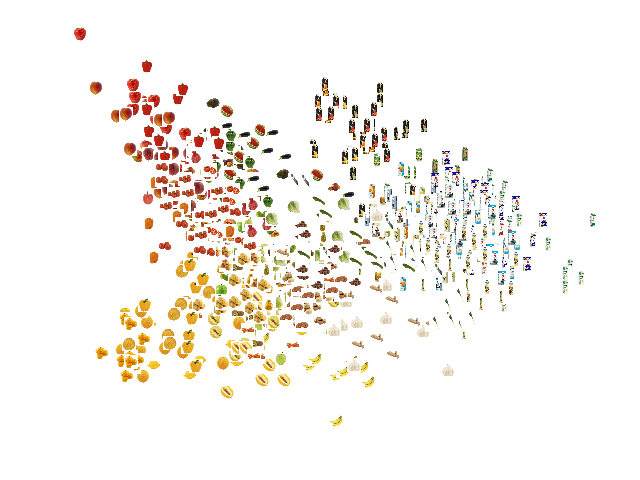
\includegraphics[width=\textwidth]{PaperB/figures_and_tables/latent_space_visualizations/pca_latents_vcca_xiy_seed2.png}
         \caption{VCCA$_{x i y}$}
         \label{fig:pca_vcca_xiy}
     \end{subfigure} 
     \begin{subfigure}[b]{0.3\textwidth}
         \centering
         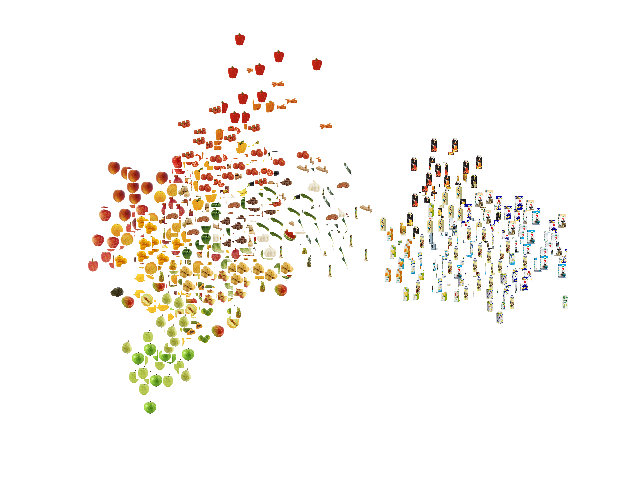
\includegraphics[width=\textwidth]{PaperB/figures_and_tables/latent_space_visualizations/pca_latents_vcca_xwy_seed2.png}
         \caption{VCCA$_{x w y}$}
         \label{fig:pca_vcca_xwy}
     \end{subfigure} 
     \begin{subfigure}[b]{0.3\textwidth}
         \centering
         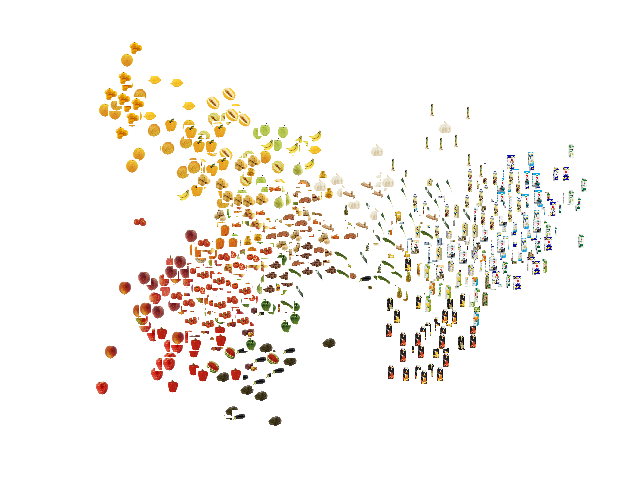
\includegraphics[width=\textwidth]{PaperB/figures_and_tables/latent_space_visualizations/pca_latents_vcca_xiwy_seed2.png}
         \caption{VCCA$_{x i w y}$}
         \label{fig:pca_vcca_xiwy}
     \end{subfigure} 
    \vspace{-2mm}
    \caption{Visualizations of the latent representations from the test set, where we plot the iconic image of the corresponding object classes. We also plot the PCA projection of the natural image features from the off-the-shelf DenseNet169 in Figure \ref{fig:pca_densenet}. All models have been initialized with the same random seed before training. %Abbreviations: VAE, Variational Autoencoder; VCCA, Variational Canonical Correlation Analysis.
    }
    \label{fig:2d_visualizations_pca}
    \vspace{-3mm}
\end{figure}
